We are concerned here with linear hardening materials which elastic domain is given by the von-Mises yield surface, under isothermal deformations in the linearized geometrical framework.
The elastic-plastic constitutive equations, derived from thermodynamics in section \ref{sec:constitutive-equations} are recalled here for convenience:

\begin{subequations}
  \begin{empheq}[left=\empheqlbrace]{align}
    \label{eq:ch5_von-Mises_yield}
    & f\(\tens{\sigma},\Acb \)= \sqrt{\frac{3}{2}}\norm{\tens{s}-\tens{Y}} - \(R(p)+\sigma^y\) \equiv 0,\quad \text{with }\tens{s}=\tens{\sigma}-\frac{1}{3}\tr \tens{\sigma} \tens{I} \\
    \label{eq:ch5_kin_hard}
    & \tens{Y}=\frac{2}{3}C\tens{\eps}^p \\
    \label{eq:ch5_iso_hard}
    & R(p)=C \: p \\
    \label{eq:elastoplastic_tangent}
    & \tens{\dot{\sigma}}=\(\Cbb - \beta\tens{m}\otimes\tens{m} \):\tens{\dot{\eps}} = \Cbb^{ep}:\tens{\dot{\eps}} \\
    \label{eq:ch5_plastic_flow}
    & \tens{m} = \frac{\tens{s}}{\norm{\tens{s}}}\\
    \label{eq:ch5_EP_acoustic}
    & A_{ij}^{ep}=  A_{ij}^{elast} -  \beta (n_k m_{ki})(m_{jl}n_l)
  \end{empheq}
\end{subequations}
In von-Mises yield function \eqref{eq:ch5_von-Mises_yield}, the Parger-Ziegler linear kinematic hardening \eqref{eq:ch5_kin_hard} is considered by removing the linear isotropic harding law \eqref{eq:ch5_iso_hard} and conversely.
Hardening parameters are thus also involved in the elastoplastic tangent modulus \eqref{eq:elastoplastic_tangent} through the parameter $\beta = \frac{6\mu^2}{3\mu +(C+R')}$ which depends on Lam\'e's constants as well.
In addition, the elastoplastic acoustic tensor \eqref{eq:ch5_EP_acoustic} is here decomposed as an elastic part $A_{ij}^{elast}$ and a plastic part depending on the direction of the plastic flow \eqref{eq:ch5_plastic_flow}.
At last, the (isotropic)elasticity tensor $\Cbb$ in equation \eqref{eq:elastoplastic_tangent} can be inverted to yield the following elastic law:
\begin{equation}
  \label{eq:ch5_elastic_inverse}
  \tens{\eps}^e = \frac{1+\nu}{E} \tens{\sigma} - \frac{\nu}{E} \tr \tens{\sigma} \tens{I}
\end{equation}
with Young's modulus $E$ and Poisson's ration $\nu$.

\subsection{Governing equations in the general case}
Reparler de la surface de charge de von-Mises, et tout et tout.
\begin{equation}
  \label{eq:ch5_conservative}
  \Ucb_t + \sum_{i=1}^D \drond{\Fcb\cdot \vect{e}_i}{x_i} = \Scb
\end{equation}
 where the conserved quantities, fluxes and source term vectors are:
\begin{equation}
  \label{eq:ch5_vectorU}
  \Ucb =\matrice{\vect{v} \\ \tens{\eps}} \quad ; \quad \Fcb\cdot\vect{e}_i = \matrice{-\frac{1}{\rho}\tens{\sigma}\cdot\vect{e}_i\\-\frac{\vect{v}\otimes\vect{e}_i +\vect{e}_i \otimes\vect{v} }{2} } \quad ; \quad \Scb = \matrice{ \vect{b} \\\tens{0}} 
\end{equation}
The governing equations of dynamics in elastic-plastic solids are written in the following quasi-linear form:
\begin{equation}
  \Qcb_t + \Absf^i \drond{\Qcb}{x_i} = \Scb \qquad \text{with: }\Absf^i = -\matrice{\tens{0}^2 & \frac{1}{\rho}\tens{I}\otimes\vect{e}_i\\ \Cbb^{ep}\cdot \vect{e}_i & \tens{0}^4}  \label{eq:ch5_quasilinear}
\end{equation}
where $\Qcb=\matrice{\vect{v}\\ \tens{\sigma}}$ and $\Cbb^{ep}=\ddroit{\tens{\sigma}}{\tens{\eps}}=\Cbb - \beta\tens{m}\otimes\tens{m}$ is the tangent modulus with $\tens{m}=\frac{\tens{s}-\tens{Y}}{\norm{\tens{s}-\tens{Y}}}$ is the flow direction and $\beta=\frac{6\mu^2}{3\mu +(C+R')}$ depends on the shear modulus $\mu$ and kinematic or isotropic hardening modulus $C$ and $R'$ (see section \ref{sec:constitutive-equations}). In particular in the arbitrary direction $\vect{n}$:
\begin{equation}
  \Qcb_t + \Jbsf \drond{\Qcb}{x_n} = \Scb  \label{eq:ch5_quasilinear_normal}
\end{equation}
where $x_n=\vect{x}\cdot\vect{n}$ and the Jacobian matrix $\Jbsf=\Absf^in_i$ arises. The left characteristic fields $\{c_K;\Lcb^K\}$ satisfy the following equation:
\begin{equation}
  \label{eq:ch5_eigen_system}
  \vect{\Lc}^K \(\Jbsf - c_K \Ibsf\) = \vect{0}
\end{equation}
As seen in section \ref{sec:characteristic_analysis}, $6$ couples of characteristic speeds $c_K$ and left eigenvectors $\Lcb^K= \[ \vect{v}^K \: , \: \tens{S}^K \]$ are determined based on those of the acoustic tensor $\tens{A}^{ep}=\vect{n}\cdot\Cbb^{ep}\cdot \vect{n}=\tens{A}^{elast} -  \beta (\vect{n}\cdot\tens{m})\otimes(\tens{m}\cdot \vect{n})$, that are $\{\omega^p;\vect{l}^p\}$ for $p=1,2,3$:
\begin{equation}
  \label{eq:ch5_left_eigenfields}
  \left\lbrace \pm \sqrt{\frac{\omega_p}{\rho}} ; \quad \[\: \pm \rho\sqrt{\frac{\omega_p}{\rho}} \vect{l}^p , -\vect{l}^p\otimes \vect{n} \:\]  \right\rbrace ,\quad p=1,2,3
\end{equation}
In addition, three independent left eigenvectors associated to the zero eigenvalue of system \eqref{eq:ch5_quasilinear_normal}, which is of multiplicity $3$, are found by solving:
\begin{equation}
  \label{eq:ch5_null_eigen}
  \tens{\sigma}^K:\(\Cbb^{ep}\cdot  \vect{n}\) =\vect{0},\quad K=1,2,3
\end{equation}

\subsection{Problems in two space dimensions}
We now focus on the solid domain bounded by $x_1 \times x_2 \times x_3 \in [0,\infty[ \times ]-\infty,\infty[ \times [-e,e]$ in a Cartesian coordinates system, where $e$ is an arbitrary length.
The solid is subject on the plane $x_1=0$ to a traction force $\vect{T}$ restricted to the $(\vect{e}_1,\vect{e}_2)$ plane, that is $T_3=0$. It is moreover assumed that all quantities except the velocity component $v_3$ depend solely on $x_1$ and $x_2$. Given the geometry of the problem, the vector $\vect{n}$ may be reduced to $\vect{e}_1$ or $\vect{e}_2$.

First, the solid is under plane strain, that is $\tens{\eps}\cdot\vect{e}_3=\vect{0}$, if for instance the velocity $v_3$ vanishes on both ends $x_3=\pm h$. In such a case, combination of the additive partition of the infinitesimal strain tensor $\tens{\eps}=\tens{\eps}^e+\tens{\eps}^p$ and \eqref{eq:ch5_elastic_inverse}, along with the kinematic condition $\eps_{33}=0$, allows to write a relation between $\sigma_{33}$ and other stress components:
\begin{equation}
  \label{eq:plane_strain_stress33}
  \sigma_{33}=\nu\(\sigma_{11}+\sigma_{22}\) - E\eps^p_{33}
\end{equation}

Conversely, if the planes $x_3=\pm e$ are traction free, a plane stress state reading $\tens{\sigma}\cdot\vect{e}_3=\vect{0}$ holds in the solid. For both plane strain and plane stress problems, the stress component $\sigma_{33}$ can then be removed from system \eqref{eq:ch5_quasilinear_normal}, leading to the unknown vector $\Qcb=[v_1,v_2,\sigma_{11},\sigma_{22},\sigma_{12}]$. The problem can then be solved in a two-dimensional setting, for which the acoustic tensor admits two distinct real eigenvalues:
\begin{subequations}
  \begin{alignat}{1}
    \label{eq:ch5_eigenAcc1}
    &\omega_1 = \frac{1}{2}\(A^{ep}_{11}+A^{ep}_{22} + \sqrt{(A^{ep}_{11}-A^{ep}_{22})^2+{4A^{ep}_{12}}^2}\) \\
    \label{eq:ch5_eigenAcc2}
    &\omega_2 = \frac{1}{2}\(A^{ep}_{11}+A^{ep}_{22} - \sqrt{(A^{ep}_{11}-A^{ep}_{22})^2+{4A^{ep}_{12}}^2}\)     
  \end{alignat}
\end{subequations}
with associated eigenvectors:
\begin{equation}
  \label{eq:ch5_eigenvectAcc}
   \vect{l}^1=[ A^{ep}_{22}-  \omega_1 \:,\: -A^{ep}_{12}] \qquad ;\qquad  \vect{l}^2=[ -A^{ep}_{12} \:,\:A^{ep}_{11}- \omega_2 ]
\end{equation}
One gets from equation \eqref{eq:ch5_left_eigenfields} that two families of waves with celerities $c_f=\pm \sqrt{\omega_1/\rho}$ and $c_s = \pm \sqrt{\omega_2/\rho}$ which are respectively referred to as \textit{fast} and \textit{slow} waves, may travel in the domain. Such waves have been identified experimentally on a thin-walled tube \cite{Clifton_exp}. Note that subtracting equations \eqref{eq:ch5_eigenAcc1} and \eqref{eq:ch5_eigenAcc2} leads to:
\begin{equation*}
  \rho c_f^2 - \rho c_s^2 = \sqrt{(A^{ep}_{11}-A^{ep}_{22})^2+{4A^{ep}_{12}}^2} \geq 0
\end{equation*}


Four left eigenfields of the Jacobian matrix then read:
\begin{subequations}
  \begin{alignat}{1}
    \label{eq:ch5_Jac_eigenfield_fast}
    &\left\lbrace \pm c_f ; \quad \Lcb^{c_f^\pm}=\[\: \pm \rho c_f \vect{l}^1 , -\vect{l}^1\otimes \vect{n} \:\]  \right\rbrace \\
  \label{eq:ch5_Jac_eigenfield_slow}
    &\left\lbrace \pm c_s ; \quad \Lcb^{c_s^\pm}=\[\: \pm \rho c_s \vect{l}^2 , -\vect{l}^2\otimes \vect{n} \:\]  \right\rbrace
  \end{alignat}
\end{subequations}
where $\Lcb^{c_f^+}$ and $\Lcb^{c_f^-}$ are associated to the right-going and left-goind fast waves respectively. The same goes for $\Lcb^{c_s^-}$ and $\Lcb^{c_s^-}$. In addition, one stationary wave associated to the zero eigenvalue of the Jacobian matrix has to be added. The left eigenvector of the corresponding characteristic field satisfies equation \eqref{eq:ch5_null_eigen} and can be taken as:
\begin{equation}
  \label{eq:ch5_null_left_eigen}
  {\Lcb^0}^T = \matrice{v_1^0 \\[5.pt] v_2^0 \\[5.pt] \sigma_{11}^0 \\[5.pt] \sigma^0_{22} \\[5.pt] \sigma^0_{12} }= \matrice{0 \\[5.pt] 0 \\[5.pt] \(C^{ep}_{121i}C^{ep}_{222j}-C^{ep}_{221i}C^{ep}_{122j}\)n_in_j \\[5.pt] \(C^{ep}_{111i}C^{ep}_{122j}-C^{ep}_{112i}C^{ep}_{121j}\)n_in_j \\[5.pt] \(C^{ep}_{112i}C^{ep}_{221j}-C^{ep}_{111i}C^{ep}_{222j}\)\frac{n_in_j}{2}} = \matrice{0 \\ 0 \\ \alpha_{11} \\ \alpha_{22} \\ \alpha_{12} }
\end{equation}

As already seen in section \ref{sec:SVK_solution}, the solutions of non-linear problems may contain shock and/or simple waves. We now focus on the second type of solutions by considering that the characteristic speeds satisfy $c_1 \geq c_f \geq c_2 \geq c_s $ and that the plastic waves celerities are decreasing functions of the stress. The first requirement implies that the characteristics do not collide while the second ensures that characteristics of plastic waves spread. Thus, the characteristic equations $\Lcb^K \cdot d\Qcb = 0$ are written:
\begin{subequations}
  %\label{eq:ch5_ODEs}
  \begin{alignat}{3}
    \label{eq:charac_fr}
    & \rho c_f \vect{l}^1 \cdot d\vect{v} - l^1_i n_j d\sigma_{ij} =0 \qquad && \text{along }\: dx/dt = c_f\\
    \label{eq:charac_fl}
    -& \rho c_f \vect{l}^1 \cdot d\vect{v} - l^1_i n_j d\sigma_{ij} =0 \qquad && \text{along }\: dx/dt = - c_f \\
    \label{eq:charac_sr}
    & \rho c_s \vect{l}^2 \cdot d\vect{v} - l^2_i n_j d\sigma_{ij} =0 \qquad  && \text{along }\: dx/dt =  c_s \\
    \label{eq:charac_sl}
    -& \rho c_s \vect{l}^2 \cdot d\vect{v} - l^2_i n_j d\sigma_{ij} =0 \qquad  && \text{along }\: dx/dt = - c_s \\
    \label{eq:charac_contact}
    &\alpha_{11}d\sigma_{11} + \alpha_{12}d\sigma_{12} + \alpha_{22}d\sigma_{22}=0 \qquad && \text{along }\: dx/dt =0 
  \end{alignat}
\end{subequations}
Integration of equations \eqref{eq:charac_fr}-\eqref{eq:charac_contact} leads to the integral curves accross simple waves in which several stress components vary, hence the name of \textit{combined stress simple waves} \cite{CRISTESCU19591605}. Following \cite{Clifton}, the method of characteristic is applied through both slow and fast waves by combining equations \eqref{eq:charac_fr}-\eqref{eq:charac_contact}.
\begin{figure}[h!]
  \centering
  \subcaptionbox{Slow simple wave \label{subfig:slowWave}}{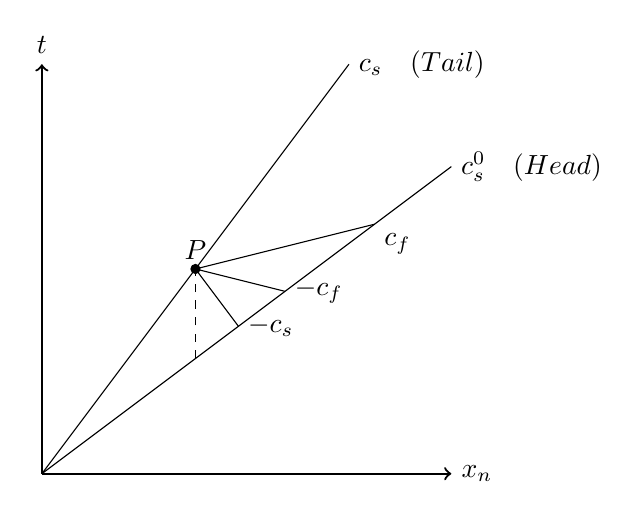
\begin{tikzpicture}[scale=1.3] 
  \newcommand\shift{5.}
  %% Slow
  \draw[thick,->] (0,0) -- (4.,0) node[right] {$x_n$};
  \draw[thick,->] (0,0) -- (0.,4) node[above] {$t$};
  % Slope = 0.75
  \draw (0,0) -- (4,3.) node [right] {$c_s^0 \quad (Head)$};
  % Slope = 4./3.
  \draw (0,0) -- (3.,4.) node [right] {$c_s \quad (Tail)$};

  \fill[black] (1.5,1.5*4./3.) circle (0.05) node [above] {$P$};
  %% Other characteristics
  % stationary
  \draw[dashed] (1.5,0.75*1.5) -- (1.5,1.5*4./3.);
  % fast plus (slope =+-0.25)
  \newcommand\px{1.5}
  \newcommand\py{1.5*4./3.}
  \draw (2.*\py-0.5*\px,1.5*\py-3.*\px/8.) node [below right] {$c_f$}-- (1.5,1.5*4./3.) ;
  % fast minus
  \draw (\py+0.25*\px,0.75*\py+3.*\px/16.) node [right] {$-c_f$} -- (1.5,1.5*4./3.) ;
  % slow minus (slope=-4./3.)
  \draw (12.*\py/25.+16.*\px/25.,9.*\py/25.+36.*\px/75.) node [right] {$-c_s$} -- (1.5,1.5*4./3.) ;
\end{tikzpicture}


%%% Local Variables:
%%% mode: latex
%%% TeX-master: "../../mainManuscript"
%%% End:
} \qquad
  \subcaptionbox{Fast simple wave \label{subfig:fastWave}}{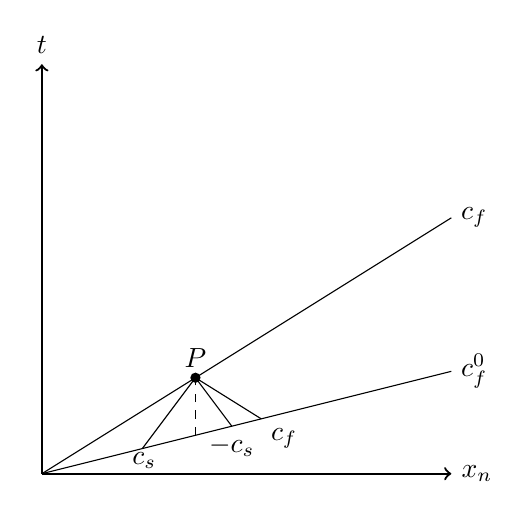
\begin{tikzpicture}[scale=1.3] 
  \newcommand\shift{5.}
  %% Fast
  \draw[thick,->] (0+\shift,0) -- (4.+\shift,0) node[right] {$x_n$};
  \draw[thick,->] (0+\shift,0) -- (0.+\shift,4) node[above] {$t$};
  % Slope = 0.25
  \draw (0+\shift,0) -- (4+\shift,1.) node [right] {$c_f^0$};
  % Slope = 5./8.
  \draw (0+\shift,0) -- (4+\shift,2.5) node [right] {$c_f$};
  
  \fill[black] (1.5+\shift,1.5*5./8.) circle (0.05) node [above] {$P$};
  %% Other characteristics
  \newcommand\pxx{1.5}
  \newcommand\pyy{1.5*5./8.}
  % stationary
  \draw[dashed] (1.5+\shift,1.5/4.) -- (\pxx+\shift,\pyy);
  % fast minus
  \draw (8.*\pyy/7.+5.*\pxx/7.+\shift,2.*\pyy/7.+10.*\pxx/56.) node [below right] {$c_f$}-- (\pxx+\shift,\pyy);
  % slow plus
  \draw (-12.0*\pyy/13.+16.*\pxx/13.+\shift,-3.*\pyy/13.+4.*\pxx/13.) -- (\pxx+\shift,\pyy);
  \node at (-12.0*\pyy/13.+16.*\pxx/13.+\shift+0.02,-3.*\pyy/13.+4.*\pxx/13.-0.12) {$c_s$};
  % slow minus
  \draw (12.0*\pyy/19.+16.*\pxx/19.+\shift,3.*\pyy/19.+4.*\pxx/19.)node [below] {$-c_s$} -- (\pxx+\shift,\pyy);
\end{tikzpicture}


%%% Local Variables:
%%% mode: latex
%%% TeX-master: "../../mainManuscript"
%%% End:
}
  \caption{The method of characteristics through slow and fast simple waves in the $(x_n,t)$ plane.}
  \label{fig:ch5_charac_method}
\end{figure}
The approach consists in tracing every characteristics from some downstream point of a wave, where the state vector $\Qcb$ is known, to an upstream point where the solution is seeked. Figures \ref{fig:ch5_charac_method}\subref{subfig:slowWave} and \ref{fig:ch5_charac_method}\subref{subfig:fastWave} show examples for slow and fast simple waves in which the state is supposed known along the \textit{head waves}, travelling at speeds $c_s^0$ and $c_f^0$, and the solution is looked for at the point $P$ lying on the \textit{tail wave}. 

\subsection{Integral curves through simple waves}
Adding equations \eqref{eq:charac_fr} and \eqref{eq:charac_fl} yields:
\begin{equation}
  l_i^1 n_j d\sigma_{ij}=0
\end{equation}
In particular, for a vector $\vect{n}$ that is restricted to the axis of the $(\vect{e}_1,\vect{e}_2)$ plane, one gets:
\begin{subequations}
  \begin{alignat}{2}
    \label{eq:sigSlow_n=e1}
    & d\sigma_{11} = - \frac{l^1_2}{l_1^1} d\sigma_{12} = \psi^s_{1}d\sigma_{12} && \qquad \text{for } \:\vect{n}=\vect{e}_1 \\
    \label{eq:sigSlow_n=e2}
    & d\sigma_{22}=- \frac{l_1^1}{l_2^1}  d\sigma_{12} = \psi^s_{2}d\sigma_{12} && \qquad \text{for } \:\vect{n}=\vect{e}_2
  \end{alignat}
\end{subequations}
It both cases, one component of the stress tensor does not appear in this equation. However, using the characteristic equation related to the contact wave \eqref{eq:charac_contact}:
\begin{subequations}
  \begin{alignat}{2}
    \label{eq:sigContact_n=e1}
    & d\sigma_{22} = -\frac{\psi^s_{1}\alpha_{11}+\alpha_{12}}{\alpha_{22}}d\sigma_{12} && \qquad \text{for } \:\vect{n}=\vect{e}_1 \\
    \label{eq:sigContact_n=e2}
    & d\sigma_{11}= -\frac{\psi^s_{2}\alpha_{22}+\alpha_{12}}{\alpha_{11}} d\sigma_{12} && \qquad \text{for } \:\vect{n}=\vect{e}_2
  \end{alignat}
\end{subequations}

Conversely, subtraction of equations \eqref{eq:charac_fr} and \eqref{eq:charac_fl} leads to:
\begin{equation}
  \label{eq:vSlow}
  dv_1 = \psi^s_{1}dv_2 = \frac{1}{\psi^s_2}dv_2
\end{equation}
Introduction of equations \eqref{eq:vSlow} and \eqref{eq:sigSlow_n=e1} in the characteristic equation \eqref{eq:charac_sl} further yields (in the direction $\vect{e}_1$) after simplification:
\begin{equation}
  \label{eq:4}
  dv_1 = -\frac{d\sigma_{11}}{\rho c_s^2} \quad ;\quad  dv_2 = -\frac{d\sigma_{12}}{\rho c_s^2}
\end{equation}
Analogously, for the direction $\vect{e}_2$:
\begin{equation}
  \label{eq:4}
  dv_1 = -\frac{d\sigma_{12}}{\rho c_s^2} \quad ;\quad  dv_2 = -\frac{d\sigma_{22}}{\rho c_s^2}
\end{equation}

Similar equations involving $\vect{l}^2$ and $c_f$ instead of $\vect{l}^2$ and $c_s$ are obtained for right-going fast simple waves. Thus, introducing $\psi^f_1=-l_2^2/l_1^2$ and $\psi^f_2=-l_1^2/l_2^2$, the equations satisfied through slow and fast simples waves are summarized in table \ref{tab:simpleWavesEquations}.
\begin{table}[h!]
  \centering
  \begin{tabular}{cc|ccN}
    \hline
    \multicolumn{2}{c}{Right-going slow wave} \vline& \multicolumn{2}{c}{Right-going fast wave} & \\
    $\vect{n}=\vect{e}_1$ & $\vect{n}=\vect{e}_2$ & $\vect{n}=\vect{e}_1$ & $\vect{n}=\vect{e}_2$&\\
    \hline
    \hline
    $dv_1 = -\frac{d\sigma_{11}}{\rho c_s^2}$ &  $dv_1 = -\frac{d\sigma_{12}}{\rho c_s^2}$ &$dv_1 = -\frac{d\sigma_{11}}{\rho c_f^2}$ &  $dv_1 = -\frac{d\sigma_{12}}{\rho c_f^2}$ &\\ [8pt]
    $dv_2 = -\frac{d\sigma_{12}}{\rho c_s^2}$ & $dv_2 = -\frac{d\sigma_{22}}{\rho c_s^2}$ & $dv_2 = -\frac{d\sigma_{12}}{\rho c_f^2}$ & $dv_2 = -\frac{d\sigma_{22}}{\rho c_f^2}$& \\ [8pt]
    $d\sigma_{11} = \psi^s_{1}d\sigma_{12}$&$d\sigma_{11}= -\frac{\psi^s_{2}\alpha_{22}+\alpha_{12}}{\alpha_{11}} d\sigma_{12}$ &  $d\sigma_{11} = \psi^f_{1}d\sigma_{12}$&$d\sigma_{11}= -\frac{\psi^f_{2}\alpha_{22}+\alpha_{12}}{\alpha_{11}} d\sigma_{12}$ & \\[8pt]
    $d\sigma_{22} = -\frac{\psi^s_{1}\alpha_{11}+\alpha_{12}}{\alpha_{22}}d\sigma_{12}$ & $d\sigma_{22}= \psi^s_{2}d\sigma_{12}$ & $d\sigma_{22} = -\frac{\psi^f_{1}\alpha_{11}+\alpha_{12}}{\alpha_{22}}d\sigma_{12}$ & $d\sigma_{22}= \psi^f_{2}d\sigma_{12}$ & \\[8pt]
    % & & \\
    % & & \\    
    \hline
\end{tabular}
%%% Local Variables:
%%% mode: latex
%%% TeX-master: "../manuscript"
%%% End:

  \caption{summarize for right-going waves}
  \label{tab:simpleWavesEquations}
\end{table}
The results for left-going waves are obtained by replacing minus signs with plus signs in the first two rows of table \ref{tab:simpleWavesEquations}. 

The last two rows of table \ref{tab:simpleWavesEquations} describe loading paths followed through the simple waves by means of one parameter families of curves. It is therefore obvious that, in contrast to what has been met so far, not only one but several stress components vary in a coupled manner through simple waves. These loading paths are studied in more details in the next section.



%%% Local Variables:
%%% mode: latex
%%% TeX-master: "../mainManuscript"
%%% End:
